\section{Fair Atomic Swaps}
\label{sec:fair_atomic_swap}

In this section, we propose two fair variants of the original Atomic Swap protocol, of which one is for currency exchange and the other is for American Call Options.


\subsection{Design}

\subsubsection{Difference between Currency Exchange and Options}
\label{subsubsec:diff_spot_option}

Before designing a fair Atomic Swap protocol, we summarize its design objectives.

To our knowledge, the Atomic Swap protocol is originally designed for the fair exchange between different cryptocurrencies.
However, according to our analysis, the protocol is unfair because Alice can choose to proceed or abort the swap based on the asset price, and he will not receive any penalty if he abort the swap.

The currency exchange and the American Call Option differ in Finance: The currency exchange is a type of Spots~\cite{hull1991introduction}, while the American Call Option is a type of Options.
The Spot Contract and the Option Contract aim at different application scenarios: The Spot Contract aims at exchanging the ownership of assets, while the Option Contract aims at providing the option buyer an ``option'' to trade.
More specifically, Spots and Options differ in the following aspects:

\begin{itemize}
    \item The Spot Contract is exercised immediately, while the Option Contract is exercised on or prior to a specified date in the future.
    \item The Spot Contract cannot be aborted once signed by both parties, while in the Option Contract the option buyer can abort the contract with the loss of the premium.
    \item The Spot Contract itself has no value, while the Option Contract itself has value - the premium.
\end{itemize}

\subsubsection{Atomic Swaps for Currency Exchange and American Call Options}
\label{subsubsec:design_obj}

According to Section~\ref{subsubsec:diff_spot_option}, the currency exchange-style Atomic Swaps and the American Call Option-style Atomic Swaps differ in design objectives.

\paragraph{Atomic Swaps for Currency Exchange}
For the currency exchange, both parties are not permitted to abort the contract once signed.
However, in Atomic Swaps, Alice can abort the swap by not releasing the random secret.
Therefore, we should discourage Alice to abort the swap.
To achieve this, we can use the premium mechanism as the collateral: Alice should deposit the premium besides her asset when \textbf{Initiate}.
The premium should follow that:
\textbf{Alice pays the premium to Bob if Bob refunds his asset after his timelock but before Alice's timelock.
If Alice's timelock expires, Alice can refund her premium back.}

\paragraph{Atomic Swaps for American Call Options}
For the American Call Options, the option buyer should pay for the premium besides the bought asset, regardless whether the contract is settled or aborted.
In reality, the option sellers are trustworthy - They never abort the contract.
However, in Atomic Swaps, Bob can abort the contracts like Alice.
To keep the Atomic Swap consistent with the American Call Options,
the premium should follow that: 
\textbf{Alice pays the premium to Bob if
1) Alice redeems Bob's asset before Bob's timelock, or
2) Bob refunds his asset after Bob's timelock but before Alice's timelock.
If Alice's timelock expires, Alice can refund her premium back.}











\subsection{Our protocols}


\begin{figure}
    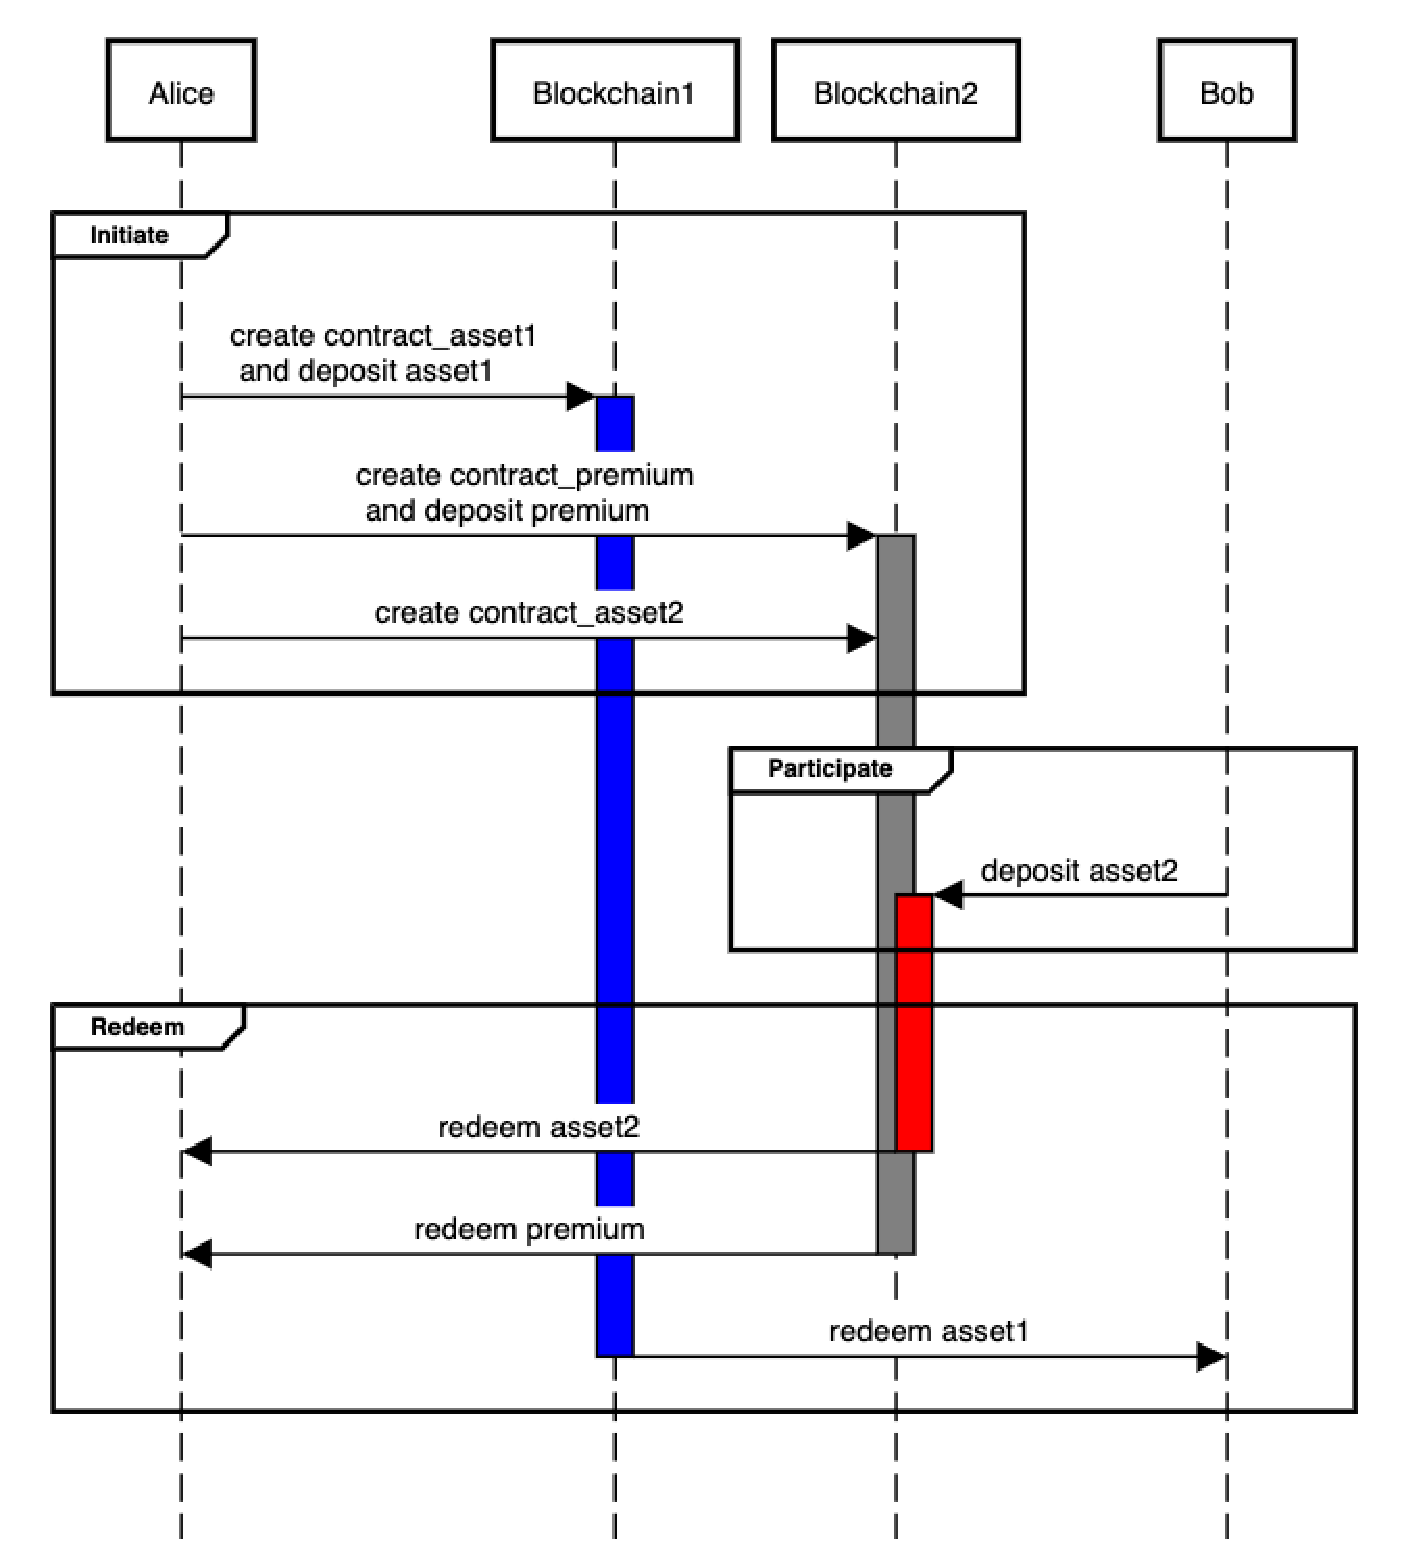
\includegraphics[width=.7\linewidth]{sequence_diagram_us_currency_exchange.eps}
    \caption{Sequence diagram of the currency exchange-style Atomic Swap.}
    \label{fig:sequence_diagram_us_currency_exchange}
\end{figure}

\begin{figure}
    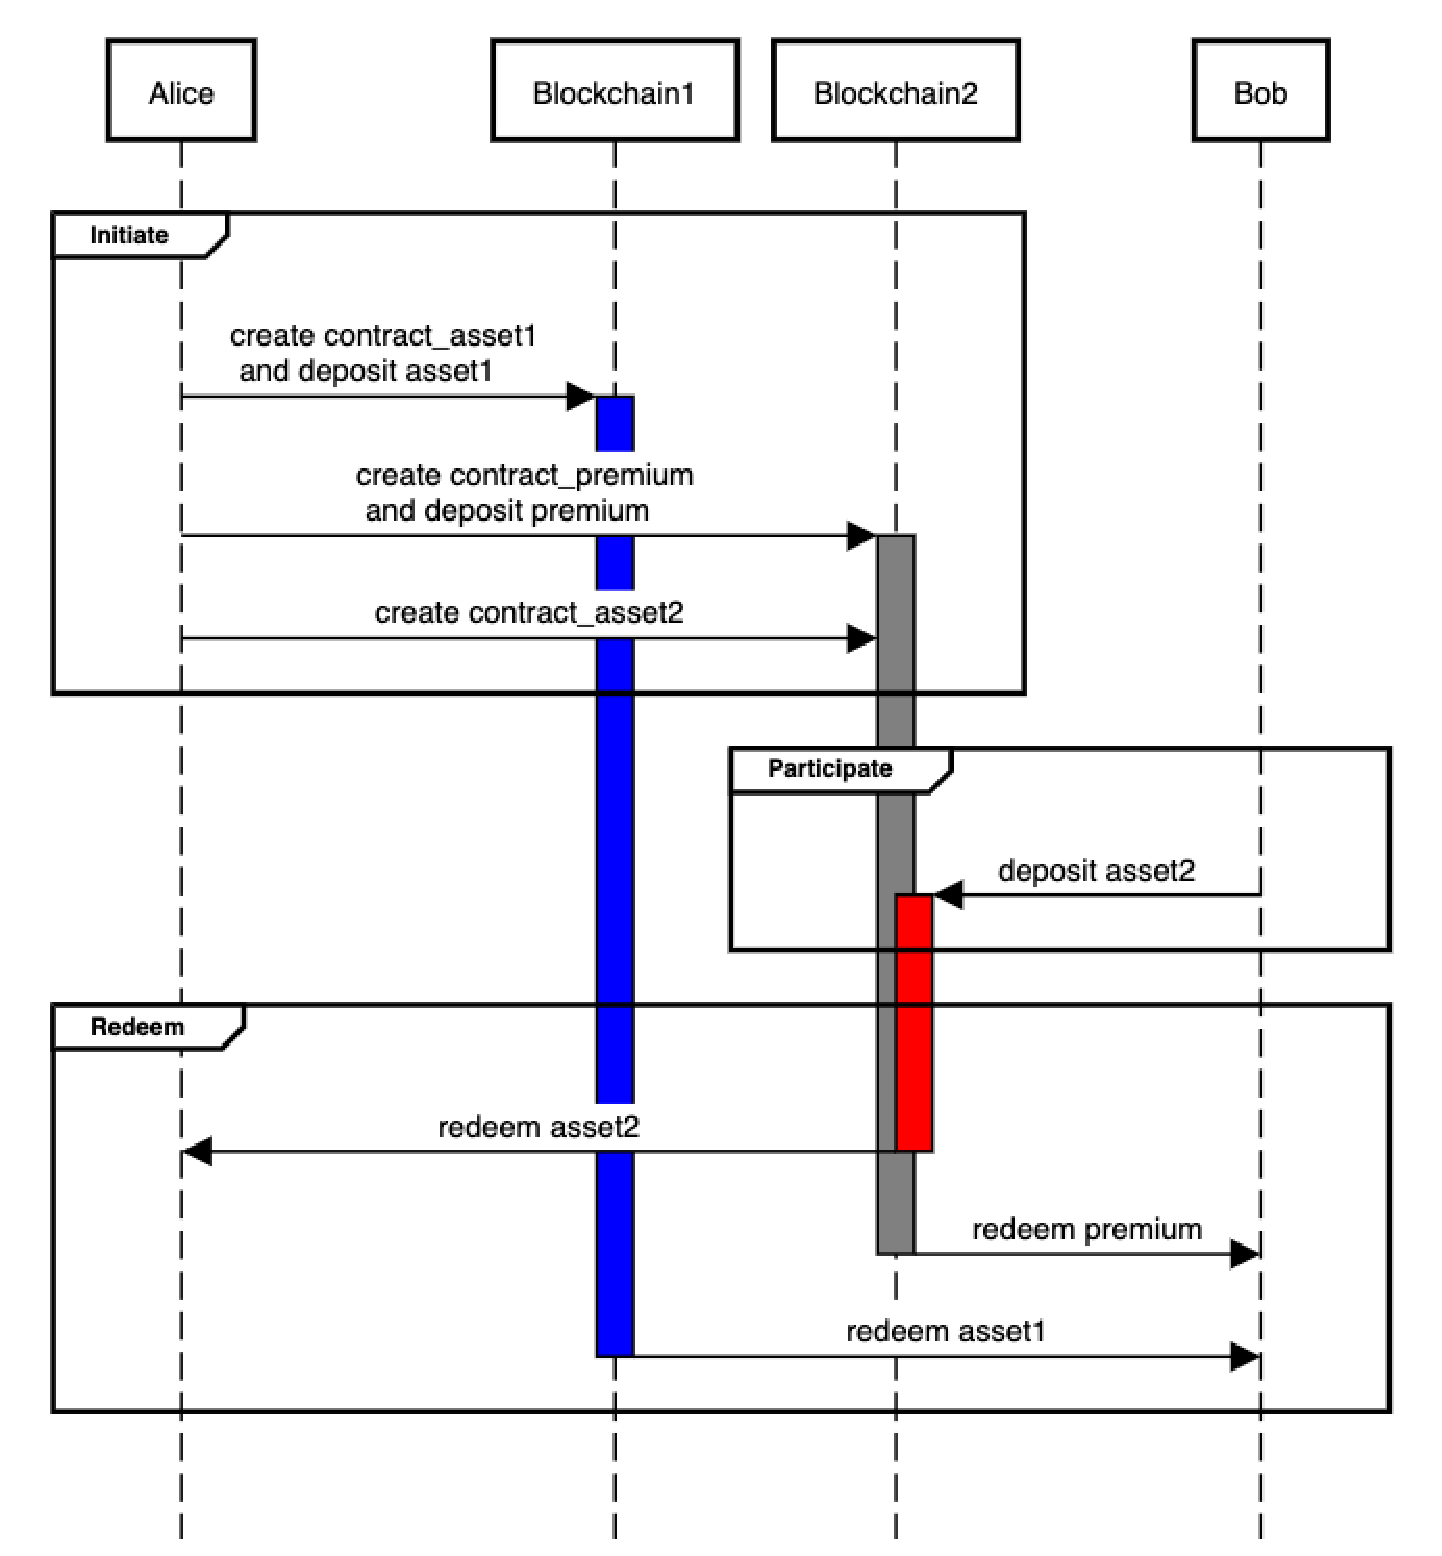
\includegraphics[width=.7\linewidth]{sequence_diagram_us_options.eps}
    \caption{Sequence diagram of the American Call Option-style Atomic Swap.}
    \label{fig:sequence_diagram_us_options}
\end{figure}


We propose two fair Atomic Swap protocols based on the original Atomic Swap protocol, but apply our design objectives in Section~\ref{subsubsec:design_obj}.
One of the two protocols is for currency exchange (shown in Figure~\ref{fig:sequence_diagram_us_currency_exchange}), and the other is for American Call Options (shown in Figure~\ref{fig:sequence_diagram_us_options}).
The two protocols are similar to each other, and only differ on the rule of premium. 

We denote our Atomic Swap protocol $\mathcal{AS}'$ as

$$\mathcal{AS}' = (x_1, Coin_1, x_2, Coin_2, pr)$$

where $pr$ is the amount of the premium measured in $Coin_2$.
In our protocols, besides $x_1$ $Coin_1$, Alice should also lock $pr$ $Coin_2$ on $BC_2$, which will be described later.

Similar to the original Atomic Swap $\mathcal{AS}$, our protocol consists of four steps:
\textbf{Initiate}, \textbf{Participate}, \textbf{Redeem} and \textbf{Refund}.
\textbf{Setup} in $\mathcal{AS}'$ is the same as in $\mathcal{AS}$, but the rest steps are different. 

\paragraph{\textbf{Initiate}}
In addition to $\mathcal{AS}$, \textbf{Initiate} in $\mathcal{AS}'$ further creates Bob's contract script $\mathcal{C}_2$, and
the associated transaction $tx_{\mathcal{C}, 2}$.

$\mathcal{C}_1$ and $tx_{\mathcal{C}, 1}$ is the same as in $\mathcal{AS}$,
while $\mathcal{C}_2$ and $tx_{\mathcal{C}, 2}$ are more sophisticated.
$\mathcal{C}_2$ contains two coherent sub-contracts $\mathcal{C}^{asset}_2$ and $\mathcal{C}^{pr}_2$.

$\mathcal{C}^{asset}_2$ is the contract for the asset $x_2$ $Coin_2$, which is the same as in $\mathcal{AS}$.
$\mathcal{C}^{pr}_2$ is the contract for the premium $pr$, which differs in the currency exchange and the American Call Options.

$\mathcal{C}^{pr}_2$ for currency exchange-style Atomic Swap $\mathcal{AS}'_{c}$ and American Call Option-style Atomic Swap $\mathcal{AS}'_{o}$ are shown below:

\begin{description}
    \item[$\mathcal{C}^{pr}_2$ in $\mathcal{AS}'_{c}$] Alice pays $pr$ to Bob with the condition:
    Bob refunds $x_2$ $Coin_2$ after $\delta_2$ and before $\delta_1$.
    If $\delta_1$ expires, Alice can refund $pr$ back.
    \item[$\mathcal{C}^{pr}_2$ in $\mathcal{AS}'_{o}$] Alice pays $pr$ to Bob with one of the two conditions:
    1) Alice redeems $x_2$ $Coin_2$ before $\delta_2$.
    2) Bob refunds $x_2$ $Coin_2$ after $\delta_2$ but before $Delta_1$ (note that $\delta_2 < \delta_1$).
    If $\delta_1$ expires, Alice can refund $pr$ back.
\end{description}

Alice published $tx_{\mathcal{C}, 1}$ on $BC_1$ and $tx_{\mathcal{C}, 2}$ on $BC_2$.
Note that Alice only triggers $\mathcal{C}_1$ and $\mathcal{C}^{pr}_2$ to execute at this stage.
Bob will trigger $\mathcal{C}^{asset}_2$ to execute by \textbf{Participate} later.

\paragraph{\textbf{Participate}}
At this stage, Bob decides whether to participate in $\mathcal{AS}'$ by auditing $tx_{\mathcal{C}, 1}$ and $tx_{\mathcal{C}, 2}$.
If Bob thinks contracts are fair, he will participate in $\mathcal{AS}'$, otherwise Bob will not and find more profitable contracts from others.
To participate in $\mathcal{AS}'$, Bob deposits $x_2$ $Coin_2$ in $\mathcal{C}^{asset}_2$, and triggers $\mathcal{C}^{asset}_2$ to execute.

\paragraph{\textbf{Redeem}}
At this stage, redeeming $x_1$ $Coin_1$ for Alice and $x_2$ $Coin_2$ for Bob in $\mathcal{AS}'$ are the same as in $\mathcal{AS}$.
But in addition, $\mathcal{C}^{pr}_2$ will work once triggering \textbf{Redeem} for $\mathcal{AS}'$.

\paragraph{\textbf{Refund}}
At this stage, refunding $x_2$ $Coin_2$ for Alice and $x_1$ $Coin_1$ for Bob are the same as in $\mathcal{AS}$.
But in addition, $\mathcal{C}^{pr}_2$ will work once triggering \textbf{Refund} for $\mathcal{AS}'$.